\begin{frame}{Future Work}
  \begin{block}{Ultrafast Group Goal}
    A novel UEM housed at UIC (Research Resources Center --- East) incorporating my laser-driven photogun
  \end{block}
  \begin{itemize}
    \item<2-> Collaboration with PNNL on new UEM 
    \item<3-> Investigate $m^{*}$ photoemission dependence
    \item<4-> Install RF compression cavity
    \item<5-> Devise and install pulse duration measurement
    \item<6-> Extend simulation for longer pulses and relativistic speeds
  \end{itemize}
\end{frame}

\begin{frame}{Summary: UEM}
\begin{block}{}
  Ultrafast Electron Microscopy is attempting to push time resolution to sub-ps time scales
\end{block}
\begin{itemize}
  \item Rose Criterion $\Rightarrow$ Require 100 electrons/pixel
  \item<2-> Short-pulse Child-Langmuir $\Rightarrow$ Require large emission area
  \begin{itemize}
    \item<2->[$\hookrightarrow$] Design/build large-aperture electron optical elements
  \end{itemize}
  \item<3-> High resolution $\Rightarrow$ Require low emittance pulses
  \begin{itemize}
    \item<3->[$\hookrightarrow$] Investigate novel photoemission sources
  \end{itemize}
  \item<4-> Must maintain pulse integrity during propagation
  \begin{itemize}
    \item<4->[$\hookrightarrow$] Developed extended AG model
    \item<4->[$\hookrightarrow$] Perl implementation available for users
  \end{itemize}
\end{itemize}
\end{frame}

\begin{frame}{Summary: Photocathode engineering}
\begin{itemize}
  \item Plasmon-enhanced photoemission
  \begin{itemize}
    \item Some cathodes produced large emission
    \item \alert{Have not} shown reduced $\Delta p_{\smallT}$
    \item Not promising for user instrument
  \end{itemize}
  \item<2-> Excited-state thermionic emission ($m^*$)
  \begin{itemize}
    \item<2-> III-Antimonides
    \item<2-> (similar III-Arsenides \footcite{liu_narrow_2005})
    \item<2-> Emission efficiency comparable to metals
    \item<2-> \alert{Have} shown reduced $\Delta p_{\smallT}$
  \end{itemize}
  \item<3-> Investigate $m^*$ dependence in other photocathode materials
\end{itemize}
\end{frame}

\begin{frame}{Thanks}
Thanks to:
\begin{columns}
  \begin{column}{.49\linewidth}
    \begin{itemize}
      \item Dept. of Energy (NNSA)
      \item National Science Foundation
      \item Dept. of Education (GAANN)
      \item Argonne Nat'l Lab (FIB)
    \end{itemize}
  \end{column}

  \begin{column}{.49\linewidth}
    \begin{columns}
      \begin{column}{1in}
        \begin{figure}
          
\includegraphics[width=0.7in]{doe}
        \end{figure}
      \end{column}

      \begin{column}{1in}
        \begin{figure}
          
\includegraphics[width=0.7in]{nsf}
        \end{figure}
      \end{column}
    \end{columns}
    %\vspace{0.4in}
    \begin{center}
      
\includegraphics[width=0.7in]{doed}
    \end{center}
  \end{column}
\end{columns}
\end{frame}

\begin{frame}{Thanks}
Thanks to:
\begin{columns}
  \begin{column}{.49\linewidth}
    \begin{itemize}
      \item Committee members
      \item Prof. W. Andreas Schroeder
      \item Ultrafast Group members
      \begin{itemize}
        \item Ben Rickman
        \item John Hogan
        \item Tuo Li
        \item Stephanie Schieffer\\(Air Force Research Lab)
      \end{itemize}
    \end{itemize}
  \end{column}
  \begin{column}{.49\linewidth}
    \begin{center}
      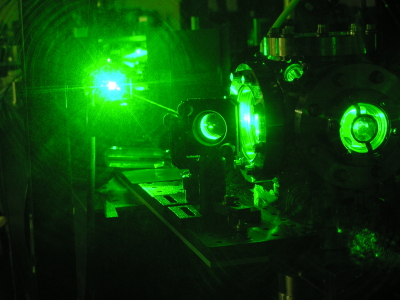
\includegraphics[width=1.3in]{Laser_Small}
    \end{center}
  \end{column}
\end{columns}
\end{frame}
